\chapter{Action stationnaire et équation d’Euler--Lagrange}

\lectureoverview{Le nom traditionnel de \emph{principe de moindre action} en masque l’idée essentielle : la trajectoire physique rend l’action stationnaire, sans nécessairement la minimiser. Nous établirons cette affirmation à partir de l’équilibre ordinaire, l’étendrons des points aux fonctions entières, déduirons l’équation d’Euler--Lagrange en discrétisant une trajectoire, puis retrouverons les équations de Newton. Enfin, les coordonnées tournantes et polaires montreront que la formulation lagrangienne ne se réduit pas à un changement de notation.}

\section{Stationnaire, pas nécessairement minimale}

Dans le nom traditionnel, c’est le mot \emph{moindre} qui prête à confusion. Une trajectoire classique ne rend pas toujours l’action minimale. Elle peut plutôt lui donner un maximum ou un point selle dans l’espace des trajectoires possibles. Le principe correct est que l’action est \emph{stationnaire} : sa variation au premier ordre s’annule.

Commençons par la question plus simple de l’équilibre. Une particule qui reste au repos n’a pas d’accélération ; la résultante des forces doit donc être nulle. Pour une force dérivant d’un potentiel unidimensionnel,
\begin{equation}
  F(x)=-\frac{dV}{dx},
  \label{eq:force-from-v}
\end{equation}
la condition d’équilibre s’écrit
\begin{equation}
  \frac{dV}{dx}=0.
  \label{eq:stationary-v-one}
\end{equation}

\begin{figure}[htbp]
  \centering
  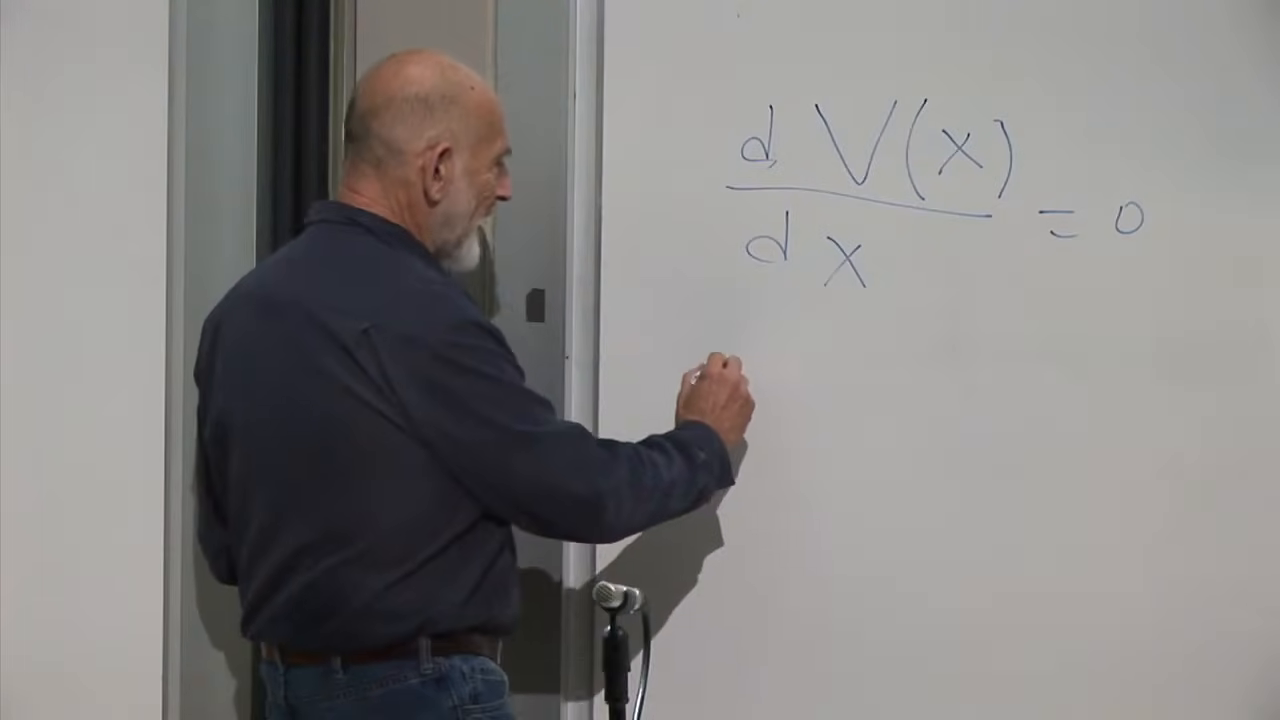
\includegraphics[width=0.74\textwidth]{lecture_03_figure_02.png}
  \caption{Condition d’équilibre en une dimension : la force s’annule là où le potentiel est stationnaire.}
  \lectureframe{00:02:51}
\end{figure}

Déplaçons maintenant la particule d’une petite quantité \(\delta x\). Au premier ordre,
\begin{equation}
  \delta V
  =V(x+\delta x)-V(x)
  =\frac{dV}{dx}\,\delta x+O(\delta x^2).
  \label{eq:first-variation-one}
\end{equation}
À l’équilibre, le terme linéaire est nul quel que soit le signe de \(\delta x\) :
\begin{equation}
  \delta V=0
  \qquad\hbox{to first order.}
  \label{eq:delta-v-zero-one}
\end{equation}
Cela ne signifie pas que \(V\) reste exactement inchangé après un déplacement fini. Cela signifie que sa variation dominante est quadratique ou d’ordre supérieur. Un minimum comme un maximum vérifie cette condition.

\begin{figure}[htbp]
  \centering
  \begin{tikzpicture}[scale=0.95,>=Latex]
    \draw[->] (-0.2,0) -- (3.35,0) node[right] {$x$};
    \draw[->] (0,-0.2) -- (0,2.25) node[above] {$V$};
    \draw[blue!65!black,thick,smooth]
      plot coordinates {(0.2,1.85) (0.75,0.85) (1.55,0.35)
                        (2.35,0.85) (3.0,1.85)};
    \fill[red!65!black] (1.55,0.35) circle (2pt);
    \node at (1.55,-0.34) {minimum};
    \begin{scope}[xshift=4.25cm]
      \draw[->] (-0.2,0) -- (3.35,0) node[right] {$x$};
      \draw[->] (0,-0.2) -- (0,2.25) node[above] {$V$};
      \draw[blue!65!black,thick,smooth]
        plot coordinates {(0.2,0.35) (0.75,1.25) (1.55,1.85)
                          (2.35,1.25) (3.0,0.35)};
      \fill[red!65!black] (1.55,1.85) circle (2pt);
      \node at (1.55,-0.34) {maximum};
    \end{scope}
  \end{tikzpicture}
  \caption{La stationnarité fixe la dérivée première, mais ne dit pas si le point est un minimum ou un maximum.}
  \label{fig:min-max-stationary}
\end{figure}

Pour plusieurs coordonnées \(q_i\), la première variation vaut
\begin{equation}
  \delta V
  =\sum_i\frac{\partial V}{\partial q_i}\,\delta q_i.
  \label{eq:first-variation-many}
\end{equation}
Si elle doit s’annuler pour tout déplacement infinitésimal indépendant
\(\delta q_i\), alors chacun des coefficients s’annule :
\begin{equation}
  \frac{\partial V}{\partial q_i}=0
  \qquad\hbox{for every }i.
  \label{eq:stationary-v-many}
\end{equation}

Il vaut mieux se représenter un potentiel à deux dimensions comme un relief vallonné que comme des montagnes russes. Un point stationnaire peut être le fond d’une vallée, le sommet d’une colline ou un point selle. En un point selle, un déplacement dans une direction fait d’abord monter, tandis qu’un déplacement dans une autre fait d’abord descendre. Le comportement de rappel peut donc être stable dans une direction et instable dans une autre, même si toutes les dérivées premières s’annulent au point considéré.

\begin{figure}[htbp]
  \centering
  \includegraphics[width=0.76\textwidth]{lecture_03_figure_06.png}
  \caption{Un point selle est stationnaire dans toutes les directions au premier ordre, bien que des déplacements voisins s’élèvent le long d’un axe et s’abaissent le long d’un autre.}
  \lectureframe{00:08:20}
\end{figure}

Dans un espace à nombreuses coordonnées, les points selle sont plus courants que les maxima ou minima purs. C’est pourquoi le terme \emph{stationnaire} reste le plus approprié. La condition
\begin{equation}
  \delta V=0
  \label{eq:equilibrium-variation}
\end{equation}
résume l’équilibre sans préjuger du comportement au second ordre.

\section{Des points aux fonctions}

La mécanique porte sur des mouvements entiers, et non sur des points d’équilibre isolés. Une trajectoire est une fonction telle que \(x(t)\), ou un ensemble de fonctions \((x(t),y(t),z(t))\). Le problème mathématique qui consiste à rendre une quantité stationnaire en faisant varier une fonction entière s’appelle le \emph{calcul des variations}. Avant de l’appliquer au mouvement, considérons trois exemples plus simples.

\subsection{Courbes les plus courtes et géodésiques}

Fixons deux points dans le plan et représentons une courbe qui les relie par \(y(x)\). Sur un petit segment,
\begin{equation}
  ds=\sqrt{dx^2+dy^2}
  =dx\sqrt{1+\left(\frac{dy}{dx}\right)^2},
  \label{eq:line-element}
\end{equation}
la dernière expression supposant \(dx>0\). La longueur totale est la fonctionnelle
\begin{equation}
  S[y]=\int_{x_0}^{x_1}
  \sqrt{1+y'(x)^2}\,dx.
  \label{eq:arc-length-functional}
\end{equation}
Les crochets indiquent que \(S\) prend une fonction entière en argument. La ligne droite est obtenue en imposant
\begin{equation}
  \delta S=0
  \label{eq:stationary-length}
\end{equation}
pour de petites variations de la courbe qui laissent ses deux extrémités fixes.

\begin{figure}[htbp]
  \centering
  \includegraphics[width=0.78\textwidth]{lecture_03_figure_07.png}
  \caption{Courbe d’essai entre deux extrémités fixes. Sa longueur est la somme des hypoténuses infinitésimales \(ds\).}
  \lectureframe{00:13:36}
\end{figure}

On peut poser la même question sur une surface courbe. Tendre une corde entre deux piquets donne une image concrète du trajet contraint le plus court. Une courbe de longueur stationnaire de ce type est une \emph{géodésique}. Dans un plan plat, c’est une ligne droite ; sur une sphère ou une surface vallonnée, ce n’est généralement pas le cas.

\subsection{Principe de Fermat}

Un rayon lumineux dans un milieu où la vitesse dépend de la position \(c(x,y)\) ne suit pas nécessairement le trajet spatial le plus court. Le temps mis pour parcourir un petit segment est la distance divisée par la vitesse locale, donc
\begin{equation}
  T[y]
  =\int_{x_0}^{x_1}
  \frac{\sqrt{1+y'(x)^2}}{c(x,y)}\,dx.
  \label{eq:fermat-functional}
\end{equation}
Le principe de Fermat impose
\begin{equation}
  \delta T=0.
  \label{eq:fermat-stationary}
\end{equation}
Lorsque \(c\) est constante, on retrouve le problème de la distance minimale. En revanche, dans un milieu d’indice variable, le trajet le plus rapide résulte d’un compromis entre la distance et la vitesse locale de propagation.

\begin{figure}[htbp]
  \centering
  \includegraphics[width=0.80\textwidth]{lecture_03_figure_08.png}
  \caption{Fonctionnelle du temps de parcours minimal pour un rayon dans un milieu où la vitesse locale de la lumière dépend de la position.}
  \lectureframe{00:22:50}
\end{figure}

Une plaisanterie d’actualité fait allusion à l’affirmation, alors récente, selon laquelle des neutrinos se seraient déplacés à une vitesse inhabituelle en Italie. L’argument de physique revient aussitôt à l’exemple fiable : dans la matière, la vitesse ordinaire de la lumière varie selon l’indice de réfraction.

\subsection{Une chaîne suspendue}

Une chaîne fixée en deux points prend la forme d’une chaînette. Chaque petit morceau contribue à l’énergie potentielle de pesanteur, si bien que le potentiel total est lui-même une intégrale le long de la chaîne. Une fois encore, les extrémités sont fixes, la forme inconnue est une fonction et une intégrale doit être stationnaire.

\begin{figure}[htbp]
  \centering
  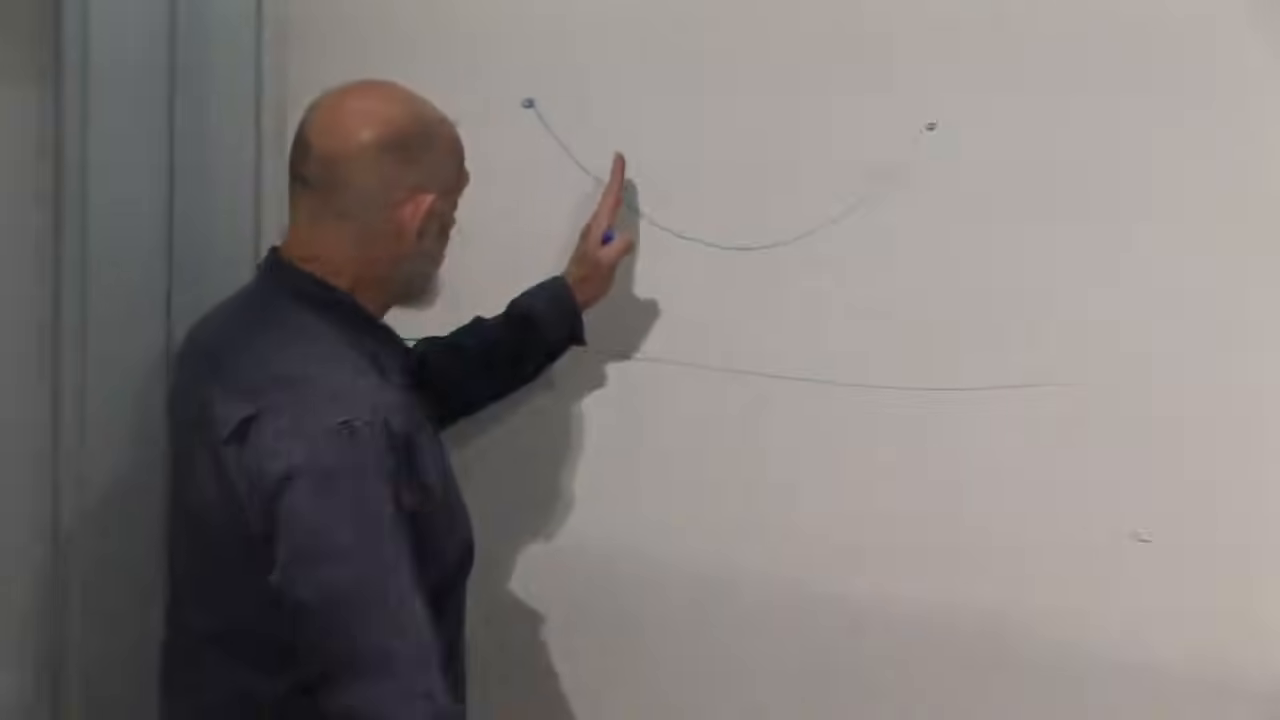
\includegraphics[width=0.76\textwidth]{lecture_03_figure_03.png}
  \caption{Chaîne suspendue entre deux appuis fixes. Sa forme stationnaire est déterminée par l’énergie potentielle de pesanteur totale.}
  \lectureframe{00:30:41}
\end{figure}

Ces exemples ont la même structure : deux extrémités fixes, une fonction qui les relie et une intégrale dont la première variation s’annule. Réduire une telle condition globale à une équation différentielle, c’est résoudre le problème variationnel.

\section{La mécanique comme problème aux limites}

On représente souvent une trajectoire avec le temps à l’horizontale, puisque \(t\) est la variable indépendante. Pourtant, en physique, il est très courant de représenter le temps vers le haut. Une digression rappelle des expériences dans lesquelles des personnes ordonnaient des images allant de la jeunesse à la vieillesse dans le sens associé à leur système d’écriture : les lecteurs de gauche à droite avaient tendance à les disposer de gauche à droite, ceux qui lisaient de droite à gauche faisaient l’inverse, et les personnes habituées à l’écriture verticale les disposaient verticalement. La plaisanterie conclut que les physiciens sont ceux qui insistent pour que le temps s’écoule vers le haut. Nous utiliserons ici l’axe horizontal conventionnel \(t\), car il permet de représenter naturellement \(x(t)\) sous forme de graphe.

Dans la formulation d’un problème à valeur initiale, les données en \(t_0\) sont
\begin{equation}
  x(t_0)=x_0,
  \qquad
  \dot x(t_0)=v_0.
  \label{eq:initial-value-data}
\end{equation}
L’équation de Newton détermine alors l’orbite ultérieure. La formulation variationnelle pose un autre problème : spécifier deux événements aux extrémités,
\begin{equation}
  x(t_0)=x_0,
  \qquad
  x(t_1)=x_1,
  \label{eq:boundary-value-data}
\end{equation}
puis déterminer la trajectoire physique qui les relie. La vitesse initiale n’est plus donnée ; elle fait partie de la solution.

\begin{figure}[htbp]
  \centering
  \includegraphics[width=0.76\textwidth]{lecture_03_figure_09.png}
  \caption{Trajectoire mécanique \(x(t)\). On peut imposer la position et la pente à une extrémité, ou les positions aux deux instants limites.}
  \lectureframe{00:27:41}
\end{figure}

La quantité à rendre stationnaire est l’\emph{action},
\begin{equation}
  A[x]=\int_{t_0}^{t_1}L(x,\dot x,t)\,dt.
  \label{eq:action-one}
\end{equation}
L’intégrande \(L\) est le \emph{lagrangien}. Il peut dépendre de la position, de la vitesse et du temps de manière explicite. Le principe de l’action s’écrit
\begin{equation}
  \delta A=0
  \label{eq:stationary-action}
\end{equation}
pour toutes les petites variations de la trajectoire vérifiant
\begin{equation}
  \delta x(t_0)=\delta x(t_1)=0.
  \label{eq:fixed-endpoint-variations}
\end{equation}
La condition aux extrémités est essentielle : nous comparons des trajectoires voisines qui relient les mêmes deux événements.

\section{Dérivation discrète de l’équation d’Euler--Lagrange}

L’action est une fonctionnelle d’une infinité de valeurs de la trajectoire. Pour rendre sa variation concrète, divisons l’intervalle de temps en pas de longueur
\(\epsilon\),
\begin{equation}
  t_n=t_0+n\epsilon,
  \qquad
  x_n=x(t_n),
  \label{eq:discrete-times}
\end{equation}
et approchons la vitesse sur le \(n\)-ième intervalle par
\begin{equation}
  v_n=\frac{x_{n+1}-x_n}{\epsilon}.
  \label{eq:discrete-velocity}
\end{equation}
L’intégrale devient la somme ordinaire
\begin{equation}
  A_\epsilon
  =\sum_{n=0}^{N-1}
  \epsilon L\left(x_n,\frac{x_{n+1}-x_n}{\epsilon}\right).
  \label{eq:discrete-action}
\end{equation}
Nous utilisons \(n\) comme indice des instants discrétisés afin de garder \(i\) disponible par la suite pour désigner des coordonnées spatiales et des particules.

\begin{figure}[htbp]
  \centering
  \includegraphics[width=0.82\textwidth]{lecture_03_figure_10.png}
  \caption{La trajectoire est remplacée par une suite d’instants discrétisés. La variation d’une hauteur intérieure ne modifie que les deux segments voisins.}
  \lectureframe{00:38:30}
\end{figure}

Faisons varier un point intérieur \(x_n\), en maintenant tous les autres \(x_k\) fixes. Seuls deux termes de la somme dépendent de \(x_n\) :
\begin{align}
  A_\epsilon\big|_{x_n}
  &=
  \epsilon L\left(x_n,\frac{x_{n+1}-x_n}{\epsilon}\right)
  \notag\\
  &\quad+
  \epsilon L\left(x_{n-1},
                  \frac{x_n-x_{n-1}}{\epsilon}\right).
  \label{eq:two-neighbor-terms}
\end{align}
La dérivation donne
\begin{align}
  0=\frac{\partial A_\epsilon}{\partial x_n}
  &=
  \epsilon\frac{\partial L_n}{\partial x_n}
  -\frac{\partial L_n}{\partial v_n}
  +\frac{\partial L_{n-1}}{\partial v_{n-1}}.
  \label{eq:discrete-el-variation}
\end{align}
Les signes opposés s’expliquent simplement par la géométrie. Élever \(x_n\) augmente la pente de l’intervalle précédent et diminue celle de l’intervalle suivant.

\begin{figure}[htbp]
  \centering
  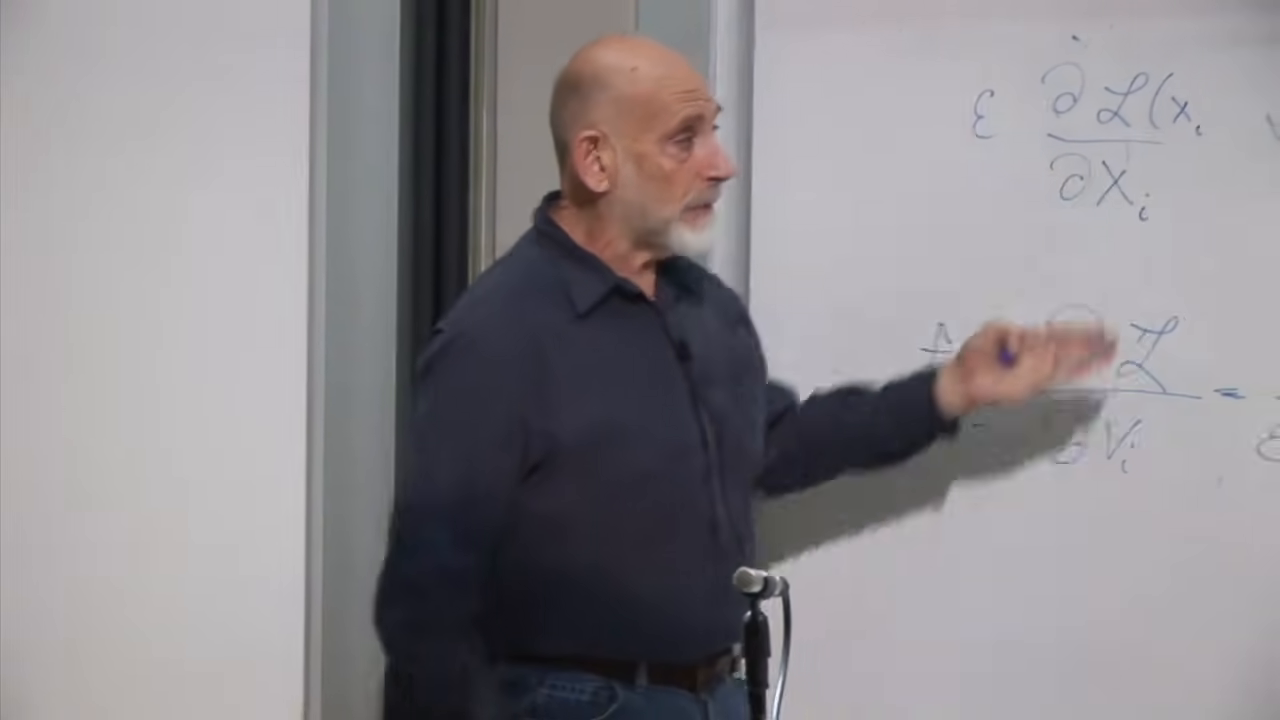
\includegraphics[width=0.74\textwidth]{lecture_03_figure_04.png}
  \caption{La dérivée directe par rapport à la position et les deux contributions des dérivées par rapport à la vitesse provenant des intervalles voisins dans la variation discrète.}
  \lectureframe{00:45:26}
\end{figure}

Réarrangeons l’équation ~\eqref{eq:discrete-el-variation} :
\begin{equation}
  \frac{1}{\epsilon}
  \left(
    \frac{\partial L_n}{\partial v_n}
    -\frac{\partial L_{n-1}}{\partial v_{n-1}}
  \right)
  =
  \frac{\partial L_n}{\partial x_n}.
  \label{eq:discrete-el}
\end{equation}
Le membre de gauche est un quotient de différences entre deux instants voisins. Lorsque \(\epsilon\to0\), la ligne brisée devient une trajectoire lisse et le quotient tend vers une dérivée temporelle :
\begin{equation}
  \boxed{
  \frac{d}{dt}\left(\frac{\partial L}{\partial\dot x}\right)
  =
  \frac{\partial L}{\partial x}}
  .
  \label{eq:euler-lagrange-one}
\end{equation}
C’est l’équation d’Euler--Lagrange.

\begin{figure}[htbp]
  \centering
  \includegraphics[width=0.78\textwidth]{lecture_03_figure_11.png}
  \caption{L’équation d’Euler--Lagrange complète, obtenue en imposant la stationnarité à chaque instant intérieur.}
  \lectureframe{00:49:25}
\end{figure}

Une fois \(L\) spécifié, l’équation ~\eqref{eq:euler-lagrange-one} fonctionne comme une machine : on dérive la fonction donnée et elle renvoie une équation différentielle pour la trajectoire.

\begin{classroomqa}
  \audiencequestion{Le résultat d’Euler--Lagrange est-il valable pour toute fonction de \(x\) et de \(\dot x\) ?\lecturetimestamp{00:49:37--00:50:24}}
  \lecturerresponse{Oui, sous réserve de la régularité nécessaire à l’existence des dérivées. Après avoir renommé sa variable indépendante \(x\) pour lui donner le rôle de \(t\), et sa fonction inconnue \(y(x)\) pour lui donner celui de \(x(t)\), l’exemple de la longueur d’arc prend exactement la même forme. Son équation d’Euler--Lagrange admet des solutions en ligne droite.}
\end{classroomqa}

\section{Retrouver les équations de Newton à partir du lagrangien}

Pour une particule se déplaçant sur une droite dans un potentiel \(V(x)\), posons
\begin{equation}
  L(x,\dot x)=T-V
  =\frac12m\dot x^2-V(x).
  \label{eq:lagrangian-tv-one}
\end{equation}
Le signe moins peut sembler étrange, car l’énergie totale est \(T+V\). Mais le lagrangien n’est pas l’énergie. Il faut vérifier si la machine d’Euler--Lagrange restitue le mouvement correct. On décline une proposition de vote fictif sur le signe : il faut vérifier le résultat, pas le soumettre au vote.

D’abord,
\begin{equation}
  \frac{\partial L}{\partial\dot x}=m\dot x.
  \label{eq:conjugate-momentum-one}
\end{equation}
C’est la quantité de mouvement. Plus généralement, la quantité de mouvement conjuguée à une coordonnée \(q\) est définie par
\begin{equation}
  p_q=\frac{\partial L}{\partial\dot q}.
  \label{eq:conjugate-momentum-general}
\end{equation}
En dérivant l’équation ~\eqref{eq:conjugate-momentum-one} par rapport au temps, on obtient
\(m\ddot x\), tandis que
\begin{equation}
  \frac{\partial L}{\partial x}
  =-\frac{dV}{dx}.
  \label{eq:lagrangian-position-derivative}
\end{equation}
L’équation d’Euler--Lagrange donne donc
\begin{equation}
  m\ddot x=-\frac{dV}{dx}=F(x),
  \label{eq:newton-from-action}
\end{equation}
qui est la deuxième loi de Newton.

\begin{figure}[htbp]
  \centering
  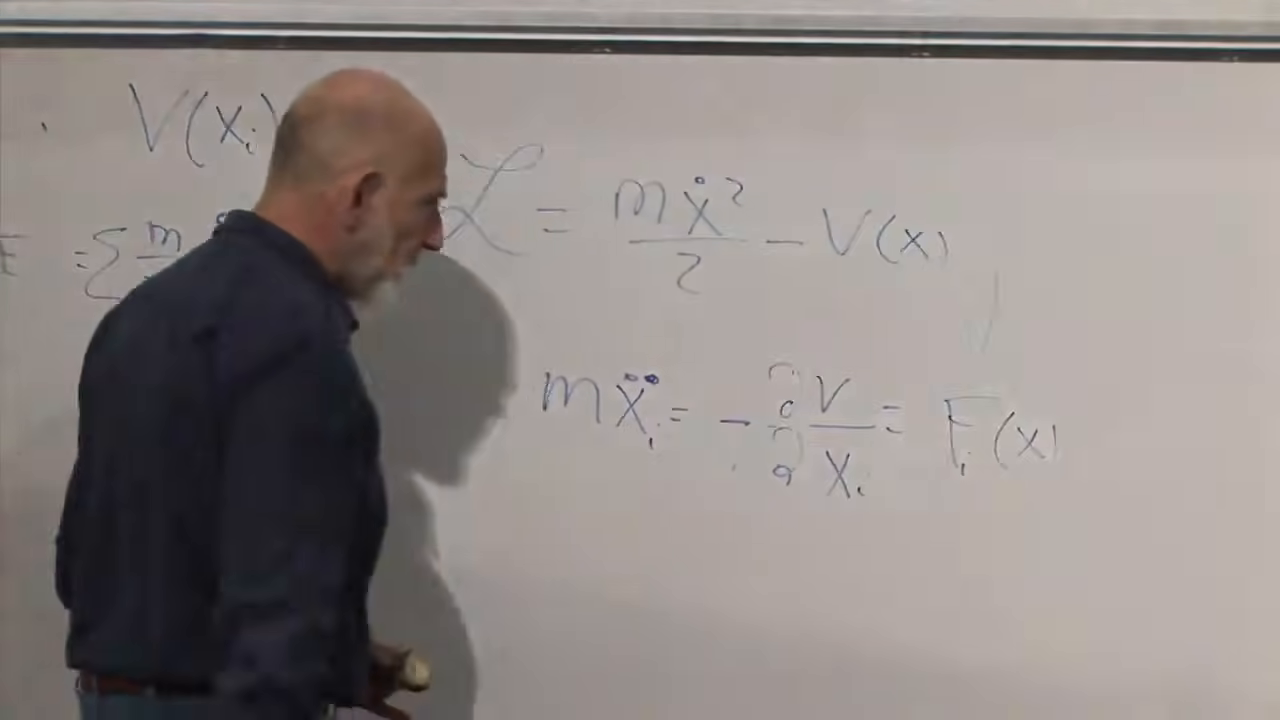
\includegraphics[width=0.80\textwidth]{lecture_03_figure_05.png}
  \caption{Énergie cinétique, énergie potentielle, \(L=T-V\) et expression par composantes de l’équation de Newton retrouvée, réunies au tableau.}
  \lectureframe{00:57:52}
\end{figure}

Pour plusieurs coordonnées \(q_i\),
\begin{equation}
  L(\mathbf q,\dot{\mathbf q})
  =\sum_i\frac12m_i\dot q_i^{\,2}-V(q_1,q_2,\ldots),
  \label{eq:lagrangian-tv-many}
\end{equation}
et il y a une équation pour chaque coordonnée :
\begin{equation}
  \frac{d}{dt}\left(\frac{\partial L}{\partial\dot q_i}\right)
  =\frac{\partial L}{\partial q_i}
  \quad\Longrightarrow\quad
  m_i\ddot q_i=-\frac{\partial V}{\partial q_i}=F_i.
  \label{eq:euler-lagrange-many}
\end{equation}
La trajectoire reste une seule courbe, mais elle se trouve désormais dans un espace des configurations de grande dimension.

\begin{classroomqa}
  \audiencequestion{N’avons-nous pas simplement remonté à rebours la loi de Newton en construisant une fonctionnelle qui restitue le résultat ?\lecturetimestamp{00:58:07--01:00:04}}
  \lecturerresponse{Ce n’est pas la manière la plus féconde d’aborder la question. Le lagrangien donne une spécification compacte du système physique : une fonction de toutes les coordonnées et de toutes les vitesses rassemble toutes ses équations du mouvement. Pour les nouvelles théories, les physiciens proposent généralement une action et en déduisent les équations, au lieu de deviner séparément chacune d’elles.}
\end{classroomqa}

Cette formulation compacte est un avantage. La liberté de choix des coordonnées en est un autre. L’affirmation selon laquelle une ligne est la plus courte ne dépend pas du fait que le plan soit décrit en coordonnées cartésiennes, polaires ou curvilignes. De même, la stationnarité de l’action est indépendante des coordonnées, même si l’expression de \(L\) et les équations obtenues pour ses composantes changent.

\section{Une particule libre vue depuis un manège}

Soient \((x,y)\) des coordonnées cartésiennes inertielles et \((X,Y)\) des coordonnées qui tournent uniformément avec une vitesse angulaire \(\omega\). Avec l’orientation choisie ici,
\begin{align}
  x&=X\cos\omega t+Y\sin\omega t,
  \notag\\
  y&=-X\sin\omega t+Y\cos\omega t.
  \label{eq:rotating-coordinate-map}
\end{align}
L’angle entre les repères est \(\omega t\).

\begin{figure}[htbp]
  \centering
  \includegraphics[width=0.76\textwidth]{lecture_03_figure_12.png}
  \caption{Axes cartésiens inertiels et en rotation uniforme. Les coordonnées tournantes du même point dépendent du temps.}
  \lectureframe{01:06:05}
\end{figure}

Le lagrangien d’une particule libre dans le repère inertiel est
\begin{equation}
  L_{\mathrm{in}}
  =\frac{m}{2}\left(\dot x^2+\dot y^2\right).
  \label{eq:free-inertial-lagrangian}
\end{equation}
Dérivons l’équation ~\eqref{eq:rotating-coordinate-map} et utilisons
\(\sin^2\omega t+\cos^2\omega t=1\). Les termes trigonométriques se combinent pour donner
\begin{align}
  \dot x^2+\dot y^2
  &=
  \dot X^2+\dot Y^2\\
  &\quad+\omega^2(X^2+Y^2)\\
  &\quad+2\omega(Y\dot X-X\dot Y).
  \label{eq:rotating-speed}
\end{align}
Ainsi,
\begin{align}
  L_{\mathrm{rot}}
  &=
  \frac{m}{2}(\dot X^2+\dot Y^2)\\
  &\quad+\frac{m\omega^2}{2}(X^2+Y^2)\\
  &\quad+m\omega(Y\dot X-X\dot Y).
  \label{eq:rotating-lagrangian}
\end{align}

\begin{figure}[htbp]
  \centering
  \includegraphics[width=0.84\textwidth]{lecture_03_figure_13.png}
  \caption{Le lagrangien transformé de la particule libre : l’énergie cinétique ordinaire, un terme quadratique centrifuge et un terme linéaire en vitesse.}
  \lectureframe{01:12:16}
\end{figure}

Le terme quadratique en coordonnées est de la forme \(-V_{\mathrm{fict}}\), où
\begin{equation}
  V_{\mathrm{fict}}
  =-\frac{m\omega^2}{2}(X^2+Y^2).
  \label{eq:centrifugal-potential}
\end{equation}
Il diminue lorsqu’on s’éloigne de l’origine et produit donc la force centrifuge
\(m\omega^2(X,Y)\).

Le dernier terme de l’équation ~\eqref{eq:rotating-lagrangian} est linéaire à la fois en les coordonnées et en les vitesses. L’équation d’Euler--Lagrange donne
\begin{align}
  m\ddot X&=m\omega^2X-2m\omega\dot Y,
  \notag\\
  m\ddot Y&=m\omega^2Y+2m\omega\dot X.
  \label{eq:rotating-equations}
\end{align}
Les termes proportionnels à \(\omega^2\) sont centrifuges ; ceux qui sont proportionnels à la vitesse sont des termes de Coriolis. Dans le plan tournant, l’écriture vectorielle est
\begin{equation}
  \mathbf F_{\mathrm{C}}
  =-2m\,\boldsymbol\omega\times\mathbf v_{\mathrm{rot}},
  \label{eq:coriolis-vector}
\end{equation}
les signes étant inversés si l’on choisit la convention d’orientation opposée.

\begin{figure}[htbp]
  \centering
  \includegraphics[width=0.84\textwidth]{lecture_03_figure_14.png}
  \caption{Équations dans le repère tournant : les termes proportionnels aux coordonnées donnent l’accélération centrifuge, tandis que les termes croisés en vitesse donnent l’accélération de Coriolis.}
  \lectureframe{01:20:20}
\end{figure}

L’essentiel n’est pas que l’algèbre disparaisse. C’est qu’une transformation de coordonnées appliquée à une seule fonction scalaire produit les deux équations couplées et les deux forces fictives.

\begin{classroomqa}
  \audiencequestion{Cette méthode fonctionne-t-elle pour des coordonnées arbitrairement curvilignes ?\lecturetimestamp{01:22:01--01:22:17}}
  \lecturerresponse{Oui. Les nouvelles coordonnées peuvent être curvilignes et même dépendre explicitement du temps, comme c’est le cas des coordonnées tournantes. Réécrivons l’action dans les nouvelles variables et appliquons la même règle d’Euler--Lagrange.}
\end{classroomqa}

\section{Coordonnées polaires et angle cyclique}

En coordonnées polaires usuelles,
\begin{equation}
  x=r\cos\theta,
  \qquad
  y=r\sin\theta.
  \label{eq:polar-map}
\end{equation}
\(r\) et \(\theta\) peuvent varier avec le temps. En dérivant et en additionnant les carrés, on obtient
\begin{equation}
  \dot x^2+\dot y^2
  =\dot r^2+r^2\dot\theta^2.
  \label{eq:polar-speed}
\end{equation}
Pour un potentiel central \(V(r)\),
\begin{equation}
  L
  =\frac{m}{2}\left(\dot r^2+r^2\dot\theta^2\right)-V(r).
  \label{eq:polar-lagrangian}
\end{equation}

\begin{figure}[htbp]
  \centering
  \includegraphics[width=0.80\textwidth]{lecture_03_figure_15.png}
  \caption{Géométrie polaire et décomposition de l’énergie cinétique entre mouvement radial et mouvement angulaire.}
  \lectureframe{01:23:30}
\end{figure}

L’équation radiale est
\begin{equation}
  m\ddot r
  =mr\dot\theta^2-\frac{dV}{dr}.
  \label{eq:radial-equation}
\end{equation}
Le premier terme est la contribution centrifuge dirigée vers l’extérieur, associée au mouvement angulaire propre de la particule.

Pour l’angle,
\begin{equation}
  \frac{d}{dt}\left(\frac{\partial L}{\partial\dot\theta}\right)
  =\frac{\partial L}{\partial\theta}=0,
  \label{eq:theta-el}
\end{equation}
car le potentiel central ne dépend pas explicitement de \(\theta\). On a donc
\begin{equation}
  \frac{d}{dt}\left(mr^2\dot\theta\right)=0,
  \qquad
  mr^2\dot\theta=\ell,
  \label{eq:angular-momentum}
\end{equation}
où \(\ell\) est le moment cinétique conservé.

\begin{figure}[htbp]
  \centering
  \includegraphics[width=0.82\textwidth]{lecture_03_figure_16.png}
  \caption{L’équation d’Euler--Lagrange pour la coordonnée angulaire a un second membre nul, ce qui met en évidence la conservation de \(mr^2\dot\theta\).}
  \lectureframe{01:29:25}
\end{figure}

L’équation angulaire donne
\begin{equation}
  \dot\theta=\frac{\ell}{mr^2}.
  \label{eq:theta-dot-angular-momentum}
\end{equation}
En substituant dans l’équation ~\eqref{eq:radial-equation}, il reste une seule équation pour \(r\) :
\begin{equation}
  m\ddot r
  =\frac{\ell^2}{mr^3}-\frac{dV}{dr}.
  \label{eq:effective-radial-equation}
\end{equation}

Une coordonnée absente de \(L\) est traditionnellement dite \emph{cyclique}, même si ce n’est pas un angle. Si \(q\) est cyclique, alors
\begin{equation}
  \frac{\partial L}{\partial q}=0
  \quad\Longrightarrow\quad
  \frac{d}{dt}\left(\frac{\partial L}{\partial\dot q}\right)=0.
  \label{eq:cyclic-conservation}
\end{equation}
sa quantité de mouvement conjuguée est conservée. On entrevoit ainsi le lien général entre symétrie et loi de conservation.

\section{Questions sur le sens, l’énergie et la portée}

Les questions qui suivent mettent en évidence où réside le contenu profond du formalisme.

\begin{classroomqa}
  \audiencequestion{Existe-t-il une raison indépendante de parvenir au lagrangien, au-delà du fait qu’il donne les bonnes équations classiques ?\lecturetimestamp{01:33:25--01:35:07}}
  \lecturerresponse{Historiquement, plus d’un siècle de mécanique classique a montré que les particules, les ondes et les champs électromagnétiques pouvaient tous être décrits sous cette forme. Au niveau classique, ce succès accumulé est un fait empirique sur la manière dont les lois s’organisent. L’explication plus profonde vient de la mécanique quantique et sera abordée plus tard.}
\end{classroomqa}

\begin{classroomqa}
  \audiencequestion{Dans le lagrangien du repère tournant, peut-on attribuer au terme linéaire en vitesse une énergie cinétique ou potentielle ordinaire ?\lecturetimestamp{01:35:08--01:36:23}}
  \lecturerresponse{Non. La quantité conservée associée aux translations temporelles s’obtient par la construction hamiltonienne ; on ne peut pas interpréter chaque terme de \(L\) comme une énergie cinétique ou potentielle. Dans l’équation ~\eqref{eq:rotating-lagrangian}, le terme linéaire en vitesse s’élimine de \(\sum_a\dot q_a\,\partial L/\partial\dot q_a-L\). Le formalisme hamiltonien organisera cela de façon systématique.}
\end{classroomqa}

En effet, puisque \(L_{\mathrm{rot}}\) ne dépend pas explicitement du temps,
\begin{equation}
  \begin{aligned}
    H_{\mathrm{rot}}
    &=\dot X\frac{\partial L}{\partial\dot X}
     +\dot Y\frac{\partial L}{\partial\dot Y}-L\\
    &=\frac{m}{2}(\dot X^2+\dot Y^2)
     -\frac{m\omega^2}{2}(X^2+Y^2)
  \end{aligned}
  \label{eq:rotating-hamiltonian-preview}
\end{equation}
est conservée. C’est l’intégrale de Jacobi dans le repère tournant, et non la même valeur numérique de l’énergie que celle attribuée par l’observateur inertiel. Un changement de coordonnées dépendant du temps ne préserve pas nécessairement la forme numérique de l’énergie.

\begin{classroomqa}
  \audiencequestion{Que se passe-t-il si la trajectoire courbe est due à la gravité ?\lecturetimestamp{01:36:30--01:37:10}}
  \lecturerresponse{Pour la gravitation newtonienne, il suffit d’utiliser \(V(r)=-GMm/r\) dans le lagrangien à force centrale. L’espace-temps courbe relève de la relativité générale et n’est pas pris en compte ici.}
\end{classroomqa}

\begin{classroomqa}
  \audiencequestion{Le potentiel centrifuge et l’énergie qui lui est associée sont-ils simplement fictifs ?\lecturetimestamp{01:37:13--01:40:14}}
  \lecturerresponse{Un observateur sur la plateforme tournante mesure les forces effectives et peut utiliser de manière cohérente la quantité conservée dans le repère tournant. Le terme \emph{fictif} signifie que ces termes viennent d’une description non inertielle, et non que leurs effets observés sont imaginaires. L’énergie elle-même n’est pas invariante sous un changement général de coordonnées dépendant du temps.}
\end{classroomqa}

\begin{classroomqa}
  \audiencequestion{Dans quelle direction pointe la force de Coriolis, qui dépend de la vitesse ?\lecturetimestamp{01:40:22--01:42:36}}
  \lecturerresponse{Elle est perpendiculaire à la vitesse dans le repère tournant ; sa norme est proportionnelle à la vitesse et à la vitesse angulaire du repère. Dans le plan, les composantes de \(\dot X\) et de \(\dot Y\) s’échangent avec des signes opposés, comme dans l’équation ~\eqref{eq:rotating-equations}.}
\end{classroomqa}

\clearpage
\begin{figure}[htbp]
  \centering
  \includegraphics[width=0.76\textwidth]{lecture_03_figure_17.png}
  \caption{Structure des composantes croisées en vitesse : la force de Coriolis est perpendiculaire à la vitesse dans le repère tournant.}
  \lectureframe{01:41:40}
\end{figure}

\begin{classroomqa}
  \audiencequestion{Le lagrangien de départ doit-il être écrit dans un repère inertiel ?\lecturetimestamp{01:42:37--01:44:00}}
  \lecturerresponse{Pour une particule libre ordinaire, la loi de Newton dans un repère inertiel fournit la forme initiale simple \(m(\dot x^2+\dot y^2)/2\). Une fois cette loi physique connue, on peut transformer l’action vers n’importe quel autre système de coordonnées. Il ne faut pas supposer indépendamment que la même formule simple de l’énergie cinétique s’applique dans un repère tournant.}
\end{classroomqa}

On trouve le même type de terme linéaire en vitesse pour une particule chargée dans un champ magnétique :
\begin{equation}
  L_{\mathrm{em}}
  =\frac12m\mathbf v^2
   +q\mathbf A(\mathbf r,t)\cdot\mathbf v
   -q\phi(\mathbf r,t).
  \label{eq:electromagnetic-lagrangian}
\end{equation}
Pour un champ magnétique uniforme perpendiculaire au plan, la jauge symétrique \(\mathbf A=\tfrac12\mathbf B\times\mathbf r\) produit un terme proportionnel à \(X\dot Y-Y\dot X\), qui a la même structure algébrique que le terme de Coriolis.

\begin{figure}[htbp]
  \centering
  \includegraphics[width=0.82\textwidth]{lecture_03_figure_18.png}
  \caption{Le terme linéaire en vitesse du repère tournant, qui motive la comparaison avec une particule chargée dans un champ magnétique uniforme.}
  \lectureframe{01:44:40}
\end{figure}

\begin{classroomqa}
  \audiencequestion{La fonction susceptible de jouer le rôle de lagrangien est-elle soumise à des contraintes autres que la régularité ?\lecturetimestamp{01:44:46--01:45:06}}
  \lecturerresponse{Oui, mais les contraintes pertinentes nécessitent un cadre plus élaboré, qui n’a pas encore été présenté ; nous les réserverons pour plus tard. Pour l’instant, l’idée centrale est de voir comment un lagrangien proposé engendre des équations et des lois de conservation.}
\end{classroomqa}

Les équations dans le repère tournant admettent aussi un mouvement circulaire : un point fixe dans le repère inertiel est vu depuis le manège comme décrivant un cercle autour de l’origine tournante. L’analogie magnétique explique alors pourquoi une particule chargée peut effectuer un mouvement cyclotron circulaire.

\begin{classroomqa}
  \audiencequestion{Une particule chargée resterait-elle sur ce cercle, ou le rayonnement ferait-il s’effondrer son orbite ?\lecturetimestamp{01:46:11--01:47:21}}
  \lecturerresponse{Les équations pour la particule seule dont il est question ici ne tiennent pas compte du rayonnement. Dès lors qu’on inclut le couplage au champ électromagnétique et la réaction de rayonnement, une charge classique accélérée peut rayonner. Le rayonnement est donc un effet physique supplémentaire, qui ne contredit pas l’orbite décrite par les équations tronquées.}
\end{classroomqa}

\begin{classroomqa}
  \audiencequestion{Quel est le rapport avec les ouragans ?
  \lecturetimestamp{01:47:30--01:47:50}}
  \lecturerresponse{Les mouvements atmosphériques à grande échelle se produisent sur la Terre en rotation ; les effets de Coriolis y sont donc importants. Une dérivation correcte relève de la météorologie et ne sera pas tentée ici.}
\end{classroomqa}

\begin{classroomqa}
  \audiencequestion{Le cadre de l’action est-il censé couvrir toutes les lois physiques, et que signifierait une véritable exception ?\lecturetimestamp{01:47:57--01:49:01}}
  \lecturerresponse{Toutes les théories fondamentales fermées connues dans le cadre de cette discussion peuvent s’organiser autour d’une action : les particules newtoniennes, les champs de Maxwell, la relativité générale et le Modèle standard. Les contre-exemples apparents, comme la traînée visqueuse, surviennent lorsqu’on omet les degrés de liberté de l’environnement. Si l’on élargit le système pour y inclure le fluide ou le bain microscopique, la description fondamentale s’inscrit de nouveau dans ce cadre. Une exception véritablement fondamentale constituerait donc une découverte majeure.}
\end{classroomqa}